\chapter{Evaluation}
This chapter will evaluate the performance and scalability of the implemented solution in terms of execution time, memory consumption, and power consumption in Section 5.1. Later on in Section 5.2 the results of the implementation are compared to the requirements from General Acoustics e.K. and finally, a comparison to similar existing ADCP solutions is presented.

\section{Performance and Scalability}
In this section, the performance of the implemented solution as well as its scalability will be tested and evaluated. First, the setup on which the tests were executed will be presented, then the assessment in terms of performance, memory consumption, and power consumption will be discussed. 
\subsection{Setup}
The measurements of the developed software were executed on three different computing stations. Two high performance devices were used to test different software configurations and acquire execution speed results while post processing old ADCP data. To test the real-time parsing of ADCP data with energy consumption in mind, a Linux driven low-power device was used.

The device with the most advanced hardware was a custom built computer with an Intel Core 6th generation i5 processor \cite{i5} over-clocked to 4.3 GHz. It had 32 GB double data rate fourth-generation (DDR4) memory \cite{ddr4} and one of the fastest solid state disk (SSD) currently available, claiming 2200 MB/s reading speed and 900 MB/s writing speed \cite{ssd}. This device was built to withstand high CPU loads, and was chosen to configure the parameters of the application and to stand as reference point for measurements with other devices.

To get performance results from a second device a Surface Book with Intel Core i7 CPU clocked at 2.6 GHz was used \cite{sb}. It had 16 GB DDR4 memory and also a fast SSD but not quite as fast as from the custom built computer (measured around 1600 MB/s read- and 600 MB/s write-speed). The results of the measurements on the Surface Book were used to compare the results from the main measuring device and, thus, gather a better impression of the overall performance of the ADCP parser application.\\
The real-time parsing requirement R1 of Section 3.1 of the software was evaluated with a BananaPro. The BananaPro has a ARM Cortex-A7 Dual-Core CPU and 1 GB DDR3 memory \cite{bpro} and runs a stripped Debian Linux derivate called Bananian Linux \cite{bananian}, it allows the configuration of the BananaPro's hardware. It has to be powered over a universal serial bus (USB). The serial port capability was enabled with a universal asynchronous receiver transmitter (UART) to USB adapter, which communicates over the RS-232 interface. To measure voltage and current flow, a USB multimeter was used \cite{mul}. Other measuring instruments to calculate a more exact energy consumption value like an oscilloscope were not available.

The different computing capabilities of the three devices allowed the evaluation of the software in terms of scalability. Scalability in this context refers to the ability of the software to adapt itself depending on the available hardware and use it accordingly.
%%%%%%%%%%%%%%%%%
\subsection{Performance}
In the evaluation of the software project, the performance of the application has an important role. Eventually the performance decides about the usability of the solution in real world scenarios and therefore, it was tested and evaluated extensively. Performance in this context relates to the execution time of the application.\\
Before any measurements were taken, the application had to be configured properly depending on the hardware and the use case. In the configuration file are a few important settings that have to be considered carefully to optimize the performance.
\begin{itemize}
\item The size of the \texttt{SequenceBuffer} (described in Section 4.2) used in the processing thread, it should at least be larger than the ADCP frame start sequence, to prevent a deadlock. Ideally, it should be larger than two times the size of the biggest ADCP frame that may be processed to prevent the processing thread from constantly auto discarding a few bytes in order to find the next start sequence.
\item The size of the Moodycamel queues used to connect the threads. If they are set wrongly the application may slow down drastically due to congestion. To avoid confusion the two queues connecting the threads were numbered: (1) is the first queue, it is a byte queue and connects the input thread to the output thread, (2) is the second queue a and contains binary messages, it connects the processing- to the output thread.
\end{itemize}

For further calculations, an average ADCP frame size of the data to be processed, was needed. The old ADCP data that was used for the performance tests had a 3992 Byte frame size for the horizontal ping, and a 992 Byte frame size for the vertical ping. The sum of both sizes was divided by two to get an average frame size of 2492 Byte. For the sake of simplicity further measurements in this report assumed an average frame size of 2500 Byte, which allowed simpler calculations.\\
Based on this average frame size, an estimate on the minimal buffer size needed was simple, it should at least be 5000 Bytes, to prevent deadlock and initial auto discarding.

The best sizes for the thread connecting queues could not be estimated easily. It could be sad that the first queue that connects the input- with the processing thread and holds the data as bytes, needs to be big enough that the processing thread can always dequeue data as needed and, thus, does not have to wait on data. Otherwise it could be assumed that the number of frames in the first queue should be equal or bigger than the number of messages in the second queue to avoid congestions.\\ 
To verify this assumptions, and get concrete numbers for the best queue sizes, a measurement was started. A bit more than one day ADCP data, exactly 150 bursts, were parsed over and over again under different queue size combinations. The execution time of each application call was written to the command line by the application and redirected into a file. The ADCP data was parsed over 1300 times, starting with very small queue sizes of 2 frames or messages in in the queues up to 400 frames or messages. \\
It had to be considered that a frame is enqueued as a number of bytes in the byte queue (1) and a message is enqueued as one object into the message queue (2). The conversion of a frame to the required number of bytes was done with the averaged frame size of 2500 Byte from above and, thus, if the first queue should contain 5 frames, the size should be set to 5 $\times$ 2500 = 12500 Byte.

\begin{figure}[hb]
\centering
      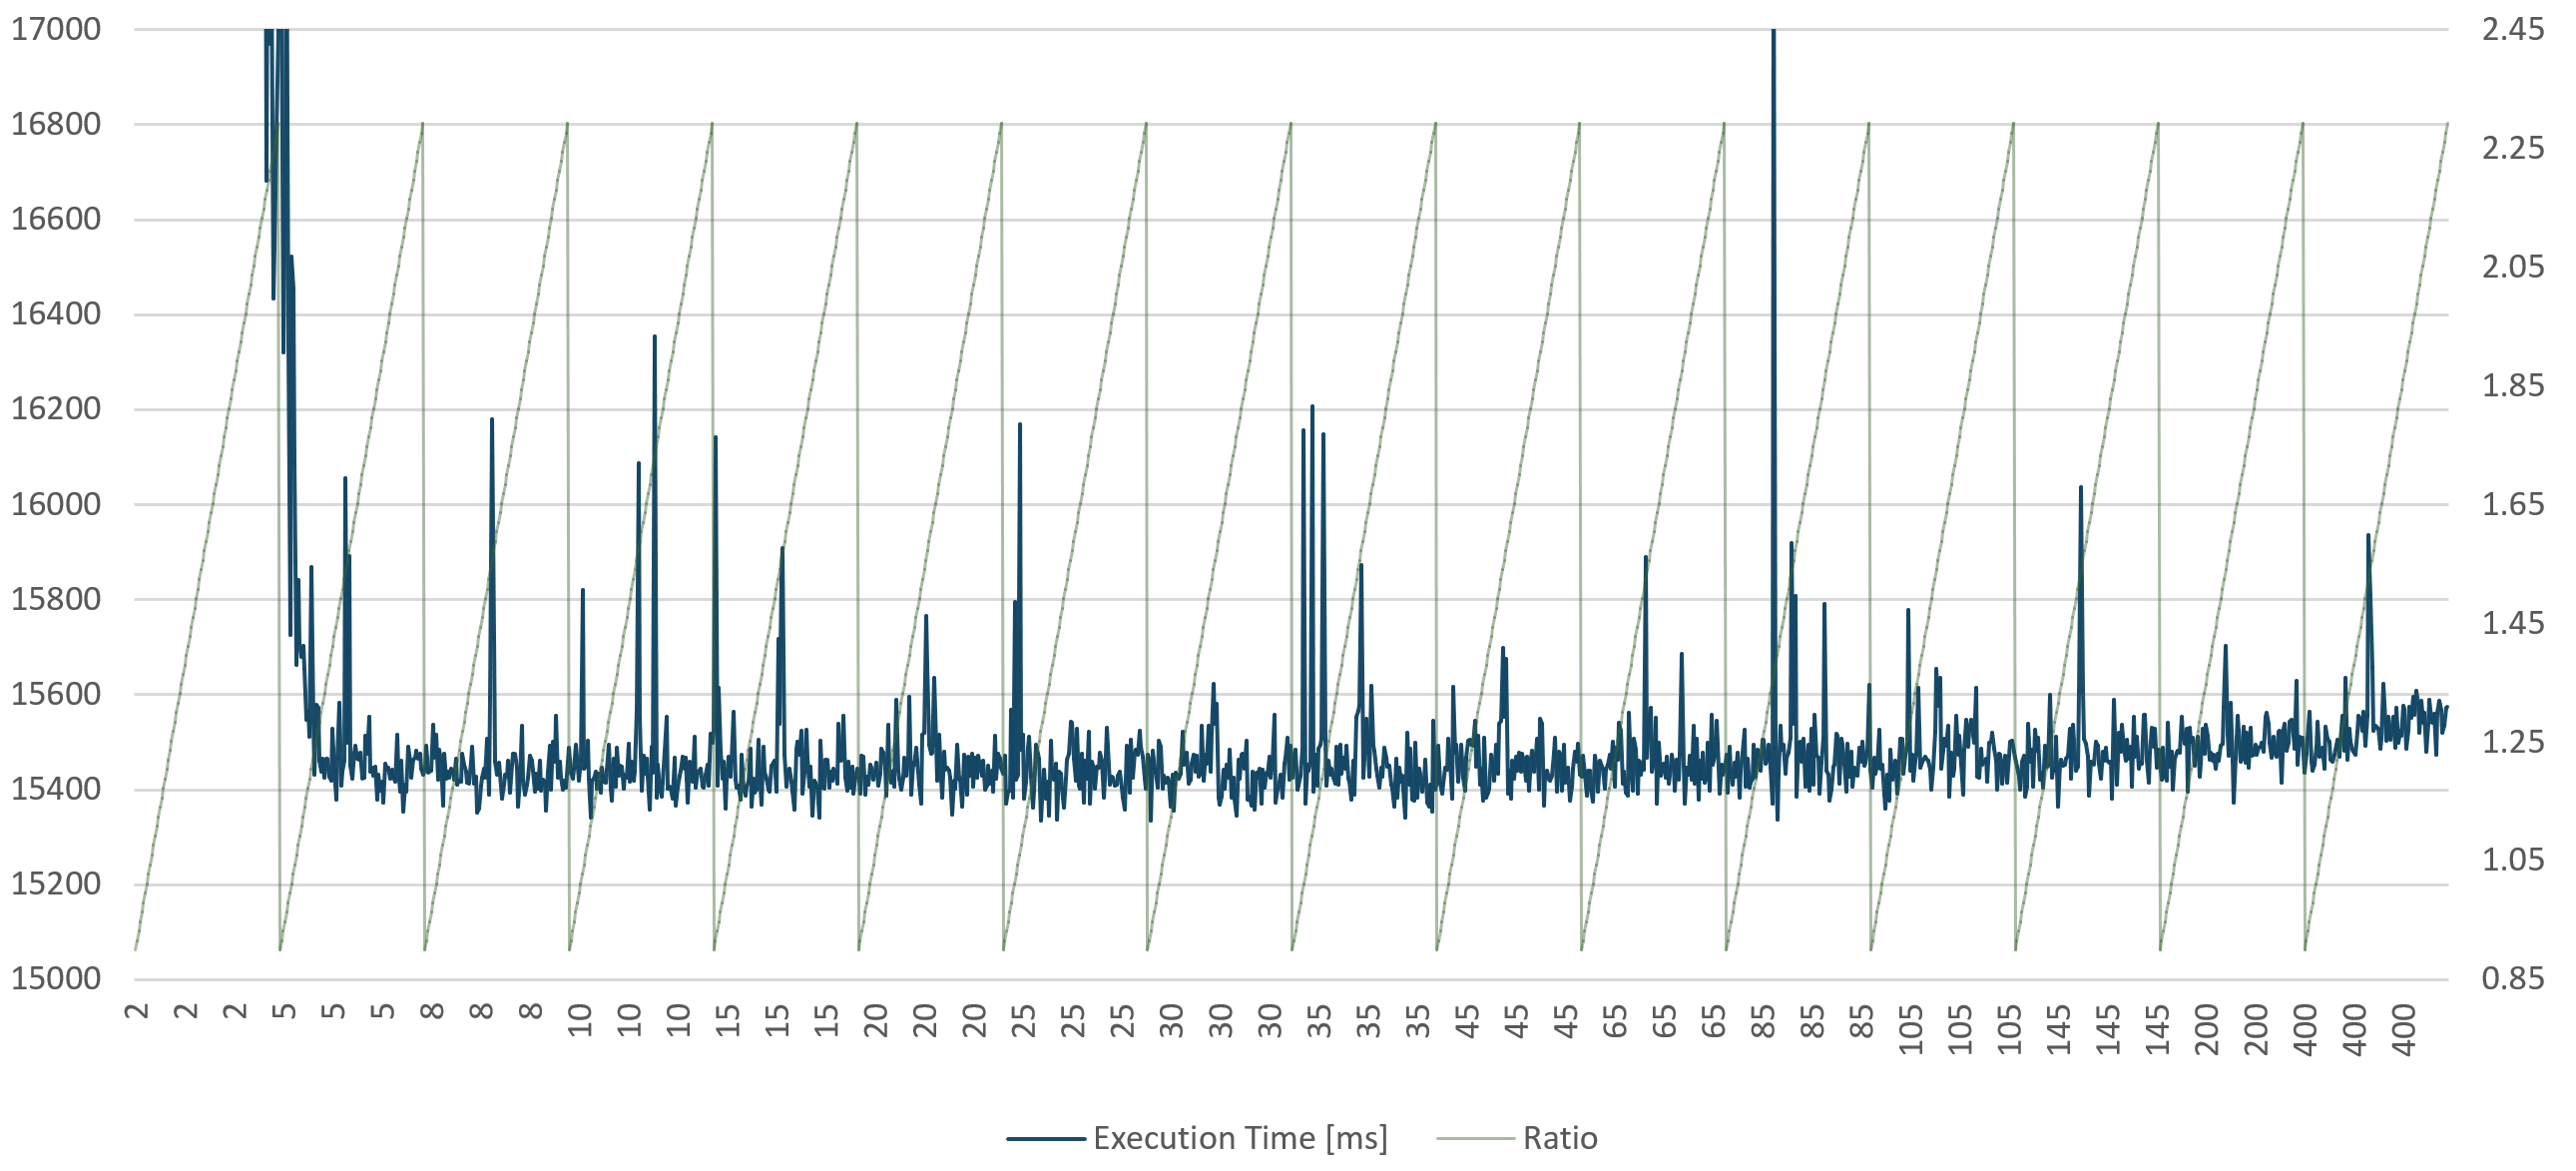
\includegraphics[width=1\textwidth]{conf_main}
        \caption{Measurement of 150 ADCP bursts under various queue configurations on a desktop computer}
\end{figure}

In the measurement, not only the number of frames in the queues were varied, but also the ratio between these queues was varied. The size of the first queue was varied between 90\% and 230\% of size from the second queue. Figure 5.1 presents the results, the light-blue zigzag line displays the ratio of the first queue (1) to the second queue (2), the darker line presents the measured time in milliseconds. The x-axis shows the number of frames in the message queue (2). It can be seen that, if the queue sizes were under five frames the measured times were visibly slower, but with values larger than five frames in the queues, the execution speed varied only around 5 percent. The outliers appeared to be random and may come from additional workload through background tasks of Windows. It can be concluded that the queue sizes should not be to low to avoid the congestion, but the selected ratio does not play a big role performance wise. Surprisingly the use of more memory due to bigger queues does not improve the performance after the minimal required queue size is reached, thus it can also be concluded that the performance limiting factor was not the memory consumption of the software.

To select a default value of the queue sizes for the configuration file, the ratio between the queues of the 50 fastest execution times were averaged. Table 5.1 shows the 20 fastest measures with its respective queue sizes. The average value over the 50 measure points was added at the end. 

\begin{table}[!]
\centering
	\begin{tabular}{l|c|c|c}
	  \hline
	  	&\textbf{Execution Time} & \textbf{Ratio (1)} & \textbf{Framenumber in(2)}\\\hline 
	  	& 15335.1 ms & 1.268 & 25\\
		& 15335.1 ms & 0.932 & 30\\
		& 15336.2 ms & 1.396 & 85\\
		& 15337.9 ms & 1.428 & 25\\
		& 15341 ms  & 1.924 & 15\\
		& 15341.4  ms & 2.004 & 35\\
		& 15341.7  ms & 1.108 & 10\\
		& 15345.9  ms & 1.86 & 15\\
		& 15346 ms & 1.764 & 30\\
		& 15346.5  ms& 1.348 & 25\\
		& 15348.5  ms& 1.812 & 20\\
		& 15352.8  ms& 1.412 & 8\\
		& 15353 ms  & 2.1	 & 5\\
		& 15353 ms  & 2.26 & 35\\
		& 15355.3 ms & 2.084 & 8\\
		& 15355.3 ms & 1.156 & 30\\
		& 15357.1 ms  ms& 1.94 & 30\\
		& 15357.7 ms & 1.684 & 10\\
		& 15358.2 ms & 2.084 & 25\\
		& 15358.3 ms & 1.684 & 15\\
		& \dots & \dots & \dots\\\hline
	  	\textbf{Average} & 15359.5 ms& 1.61 & 34.5\\ 
	  \hline
	\end{tabular}
	\caption{The 20 fastest execution times with the respective ratio and queue size}
\end{table}

To verify the measured behavior, the same test was executed on the Surface Book, Figure 5.2 presents the results in a similar graphic than already explained for Figure 5.1, it can be seen that the execution time is slower around 7 seconds, and varies much more than in Figure 5.1. The time varies between 22.5 seconds and 25.5 seconds, but a clear bias can be seen towards 22.75 second. This behavior may result from CPU throttling due to thermal issues and, thus, it can be concluded that a mobile CPU as used in the Surface Book is not the best choice for heavy data processing. Nonetheless the results confirm that the application does not depend on the amount of memory used after exceeding the minimal required queue size. They also confirm that the ratio between the queues has no big impact on the execution time as already seen in Figure 5.1. 
\vspace{1em}

\begin{figure}[h]
\centering
      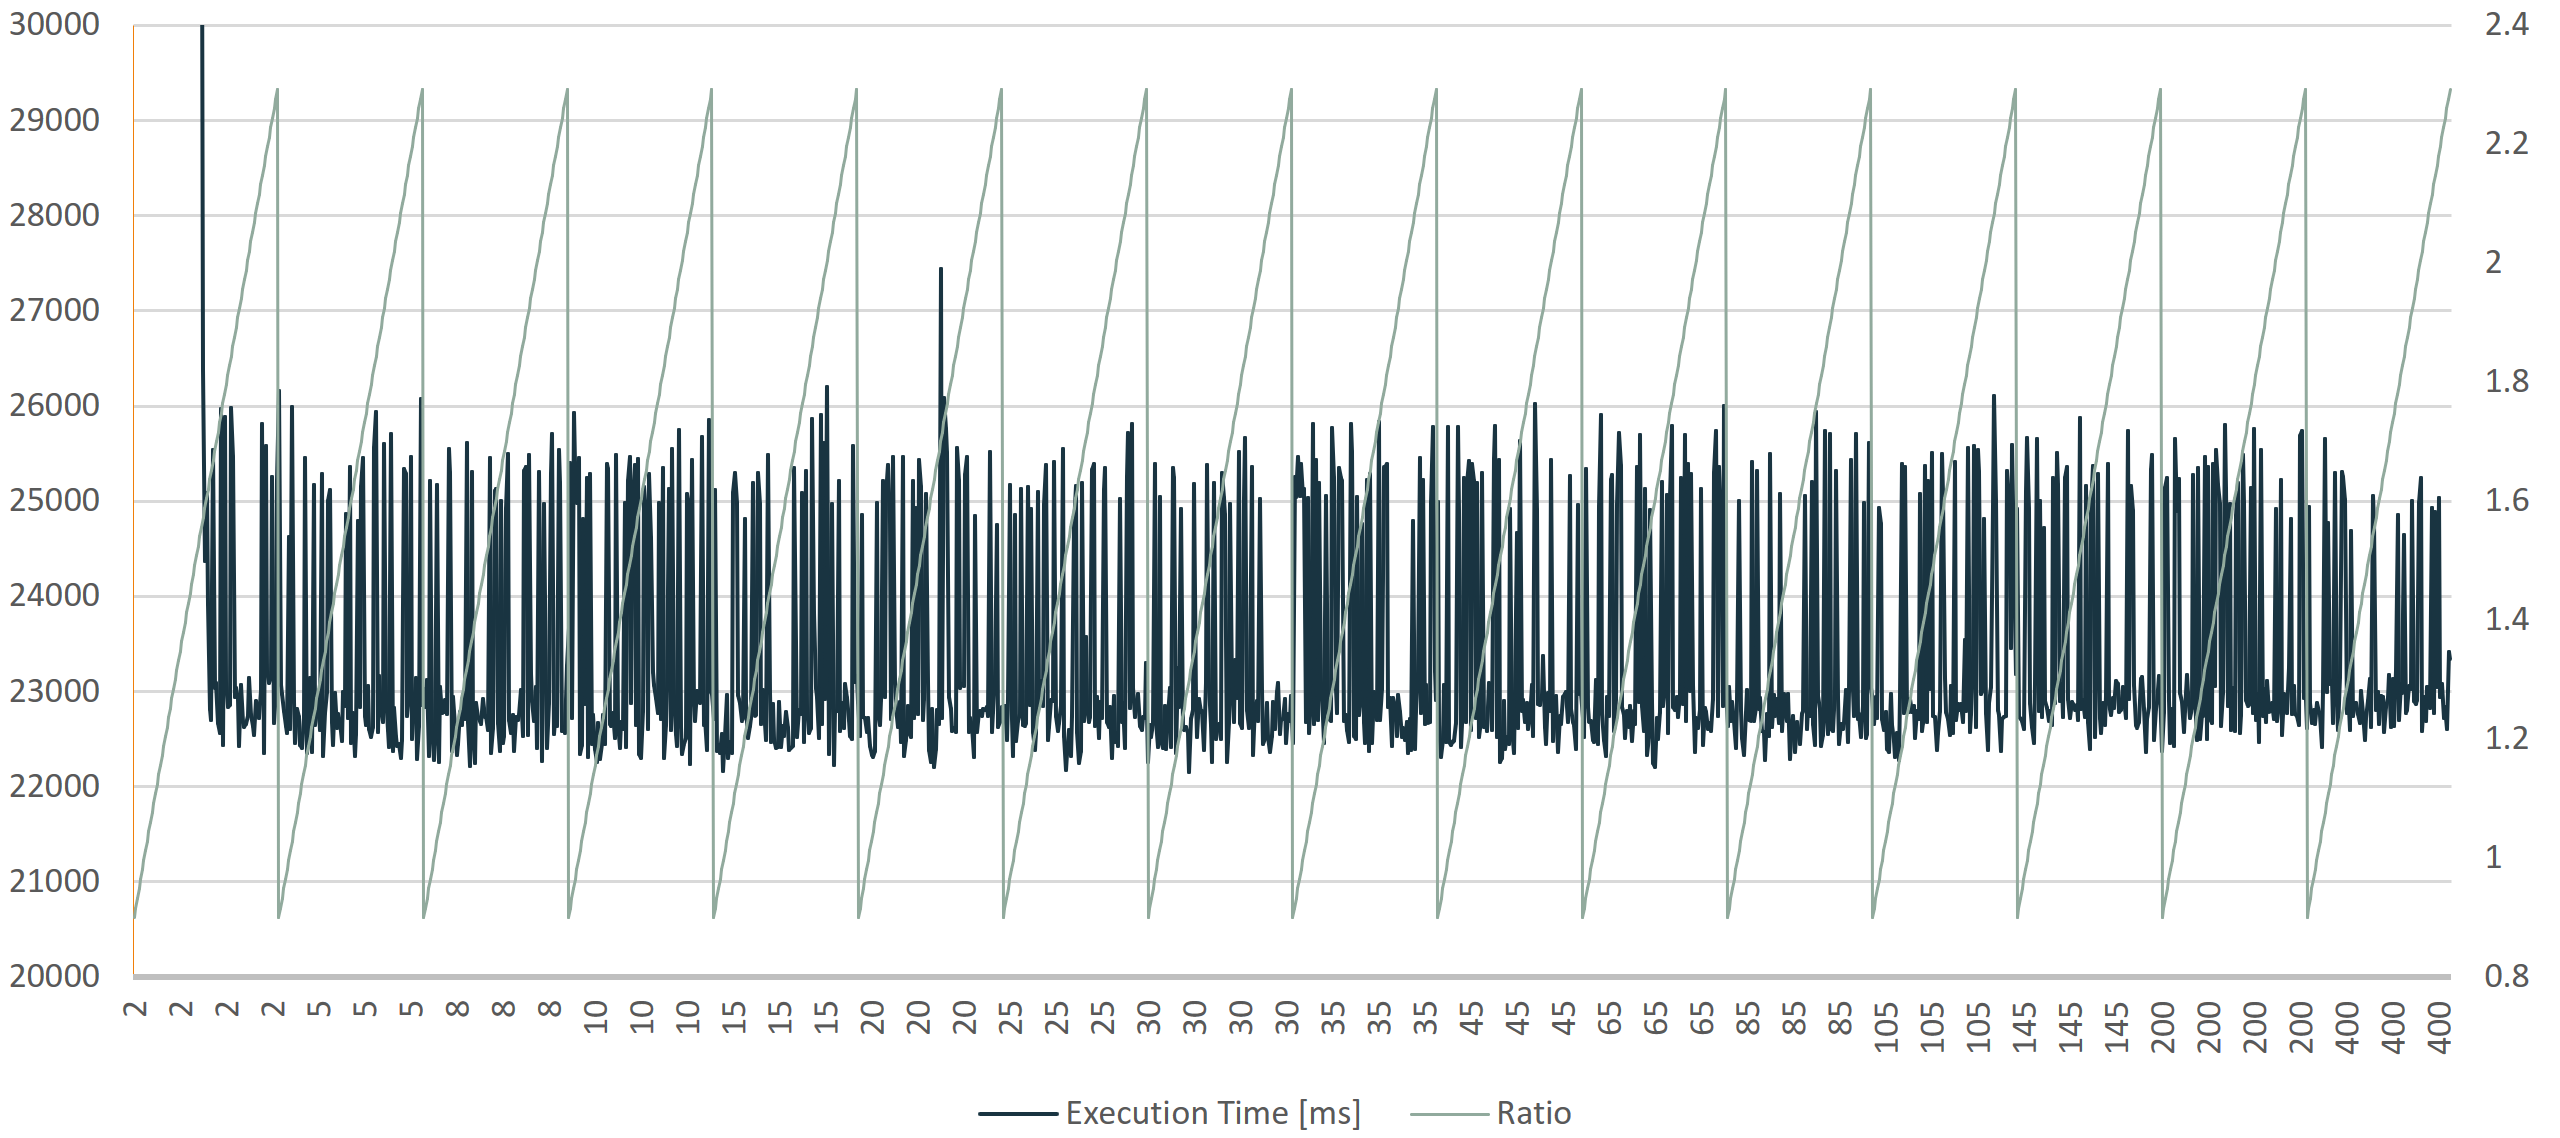
\includegraphics[width=1\textwidth]{conf_sb}
        \caption{Measurement of 150 ADCP bursts under various queue configurations on a Surface Book}
\end{figure}

To reassess the new found memory independence, a new measurement was executed. This time the fixed size ratio of 1.6 as calculated in Table 5.1, was used between the queues. Once again sizes between two and 400 frames in the message queue were measured in 90 steps five times. The averaged results are presented in Figure 5.3, it can be seen that the execution (orange line) time even gets slightly poorer if the queue sizes (on the x-axis) grow over 80 frames, which may result from slower performance of the Moodycamel queues if they are allocated to big, but remain empty most of the time.
\vspace{1em}

\begin{figure}[h]
\centering
      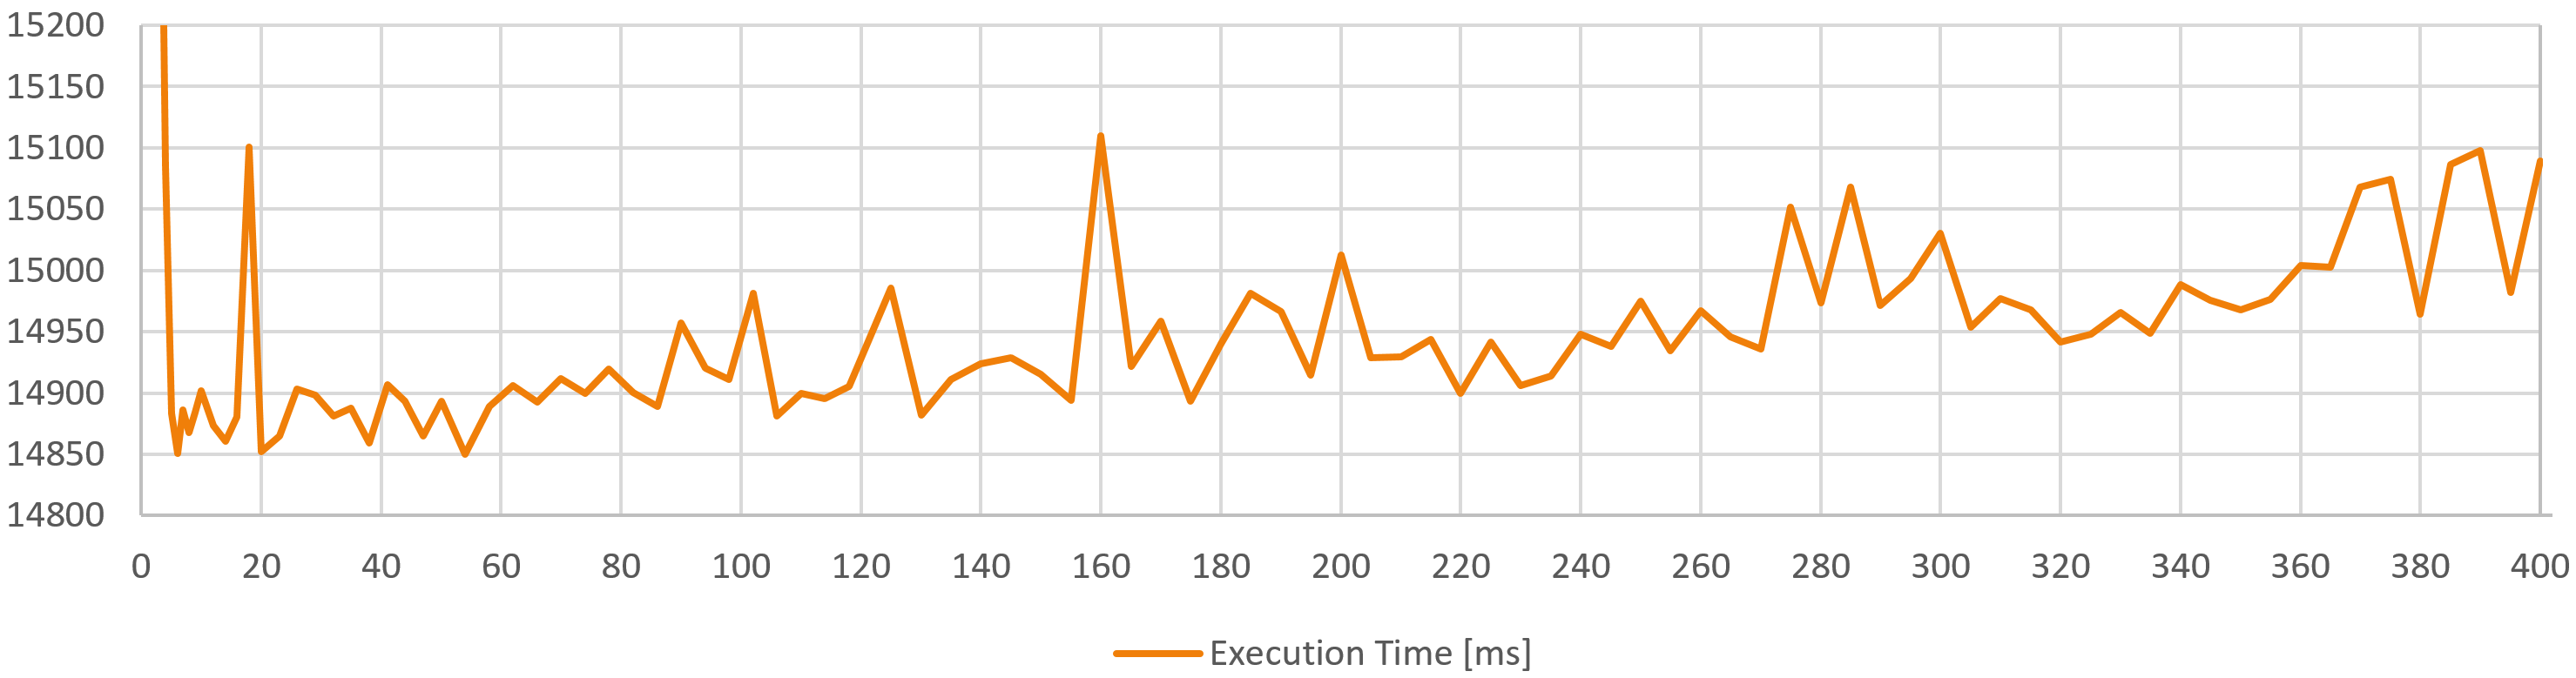
\includegraphics[width=1\textwidth]{perf_mem_1}
        \caption{Impact of extensive memory usage on the execution time}
\end{figure}

\pagebreak
After seeing that the memory consumption did not have a big impact on performance some general tests were done where different amounts of old data was parsed at a fixed configuration of 30 frames in the message queue (2) and a ratio of 1.6 for the byte queue (1). Table 5.2 presents the resulting figures. 
\vspace{2em}
\begin{table}[!h]
\centering
	\begin{tabular}{|l|c|c|}
	  \hline
	  	\textbf{Device} & \textbf{Desktop Computer} & \textbf{Surface Book}\\ \hline
	  	\textbf{10 Minutes (5 MB)} & 152 ms & 238 ms\\
	  	\textbf{1 Day (700 MB)} & 14.9 s & 20.95 s\\
	  	\textbf{1 Week (4.9 GB)} & 104.3 s & 147.4 s\\
	  \hline
	\end{tabular}
	\caption{Execution time at a fixed configuration and various amount of data on the desktop computer and the Surface Book}
\end{table}
\vspace{1em}

With this performance three years of old ADCP data could be parsed in under 5 hours, resulting in around 105 ms per 10-minutes burst. It can be concluded that this performance satisfies all needs in terms of post processing.

To complete the post processing requirement measurements, the BananaPro was also used to post-process some old ADCP data. The results shown in Table 5.3 show really slow execution times of around XXX seconds per ADCP frame. The results are understandable, as the processor has not the power to do extensive data processing and was not built for it.
\vspace{2em}
\begin{table}[!h]
\centering
	\begin{tabular}{|l|c|}
	  \hline
	  	\textbf{Device} & \textbf{BananaPro}\\ \hline
	  	\textbf{10 Minutes (5 MB)} & 8.1 s \\
	  	\textbf{1 Hour (30 MB)} & 47.8 s \\
	  \hline
	\end{tabular}
	\caption{Execution time at a fixed configuration and various amount of data on the BananaPro}
\end{table}
\vspace{1em}

The memory consumption can be ruled out as performance critical bottleneck if a queue size larger than five frames is used. The real bottleneck in the current implementation is the processing thread, on the main computer, the core running the processing thread was always busy at 100\% whereas the overall CPU load never exceeded 65\%. Currently the processing thread does all CPU intensive work, it converts the ADCP frames to ADCP ensembles containing integers and floats, then cleans the data, and converts the ensemble back to a frame and later completely to bytes. The idea of this implementation was the preparation for further processing steps. For example, if a second processing step would be implemented for wave analysis, the first processing thread would only convert the data to ADCP ensembles, and pass them to the second thread, where they would used further. In the last part of Chapter 6 a solution to improve the current design is described.

\subsubsection{Real-Time Parsing} 
The real-time processing, was tested first under Windows. A pair of virtual COM ports was used to test high data throughput with a Baud rate of 468000 Bd. This Baud rate is also used for the real ADCP communication over an RS-485 interface. The application run flawlessly consuming 5 MB memory and one percent CPU usage, even with five times of the data that would be generated by an ADCP.\\
The tests with the BananaPro had to be done over RS-232 interfaces as no appropriate RS-485 hardware was available. The RS-232 adapters used allowed a maximum Baud rate of 115200 Bd, this was just enough to receive two times the data that would normally be generated by an ADCP.\\
On the BananaPro the application used again around 5 MB memory, and burdened the CPU with a maximum of 3 percent CPU load. The reached performance is really good, as the data to be processed from a real ADCP would be lower and, thus, the CPU load would be as well lower.
\subsection{Memory Consumption}
The memory handling of the software is straight forward. Most objects are allocated on the stack and eventual memory leaks of the heap were carefully eliminated, as the software may have to run infinitely and must not grow. After all components are instantiated, the allocated memory oscillates only very little, even if the application runs idle. The reason is, that most objects of the software are rather allocated once and overwritten, than destroyed and reallocated. Another reason is, all data structures are preallocated and prohibited to grow. This circumstance means that the maximal memory consummation can be estimated before running the application.\\
\begin{figure}[h]
\centering
      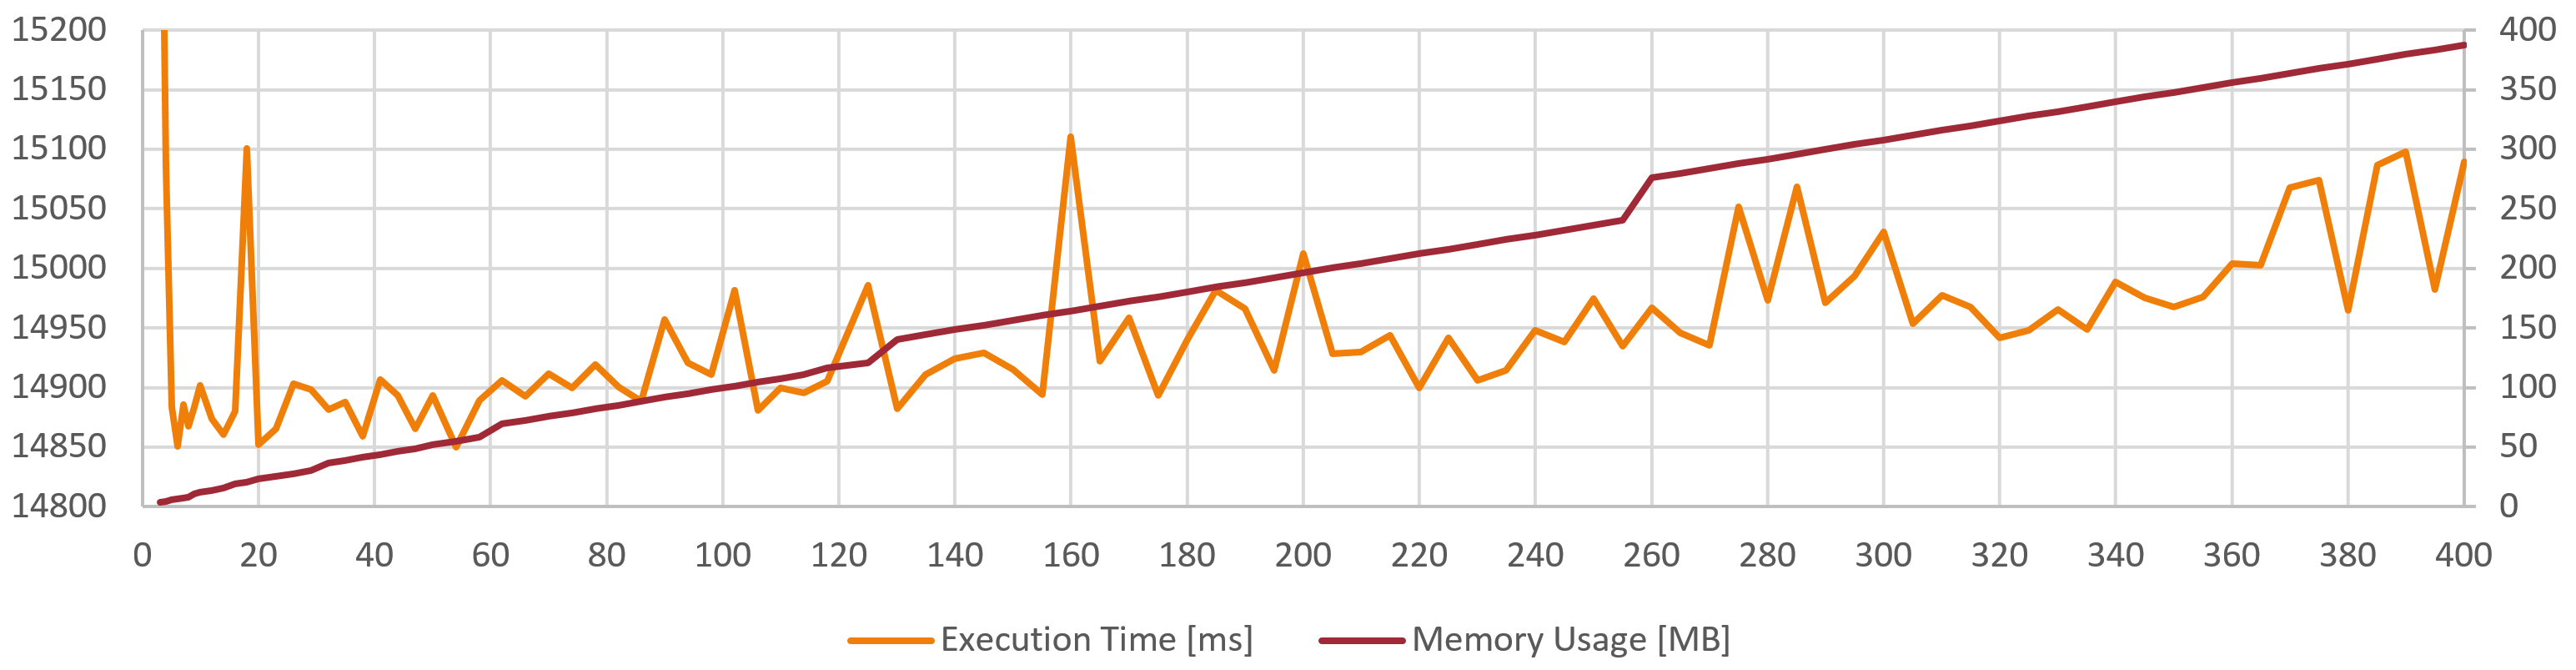
\includegraphics[width=1\textwidth]{perf_mem_2}
        \caption{Memory Consumption and execution time for various queue sizes}
\end{figure}

Figure 5.4 shows the memory consumption of the test run shown in Figure 5.3 from the previous Section 5.1.2, one can see that the memory grows equally with the preset sizes of the queues. 
%ith the average ADCP frame size of 2500 Byte calculated in Section 5.2.1 and the number of frames in the message queue it is possible to calculate the number of estimated ensembles in the system. To simplify this calculation it was assumed that only the ensembles in the byte queue from the input thread to the processing thread, as well as the message queue from the processing thread contain ensembles. The ensembles currently floating in the three threads were ignored.\\
%The estimated ensemble number was compared against the actual memory consumption. It can be seen that an ensemble in the application requires around 0.45 MB memory, 
In Figure 5.4 the red line represents the used memory of the whole application. The memory used equals more or less the number of ensembles in the  message queue. The high values are because the Moodycamel queues preallocate their memory in a way that all threads are always able to execute their desired nonblocking operation. This requires to maintain more memory than actually needed. But as seen in Section 5.1.2 the application performs perfectly with a reasonable amount of memory, for example for the calculated average queue sizes, around 30 MB memory.

\subsection{Power Consummation}
In Section 5.1.2 the performance of the software on the BananaPro was assessed in terms of speed, there, it was shown that the BananaPro is not made for batch-processing of old ADCP data, but that it is fast enough by far to process real-time data. It was also shown that the configuration for the BananaPro in real-time parsing mode works well with as few as 4-5 MB memory, and almost never exceeds CPU usage of more than 3 percent.\\ 
The missing information about the power consummation of the BananaPro was measured with the USB multimeter described in Section 5.1.1. First the voltage and current was measured when the BananaPro was idle and then while executing the application. During the measurements the power adapter was changed because the old one could only deliver 750mA at 4.9 V which lead to variations of 60 mA. With the new power adapter which could deliver up th 2.4 A, no more ups and downs could be measured. Table 5.x presents the results of the measurements with the new power adapter, with a stable voltage, and a difference of 10 mA for the current. The multimeter only had a 10 mA resolution and therefore the measurement is not very exact, but it shows at least that the power consumption does not exceed 10 mA which is a maximum 3.5 percent of the overall power consumption.

\begin{table}[h]
	\centering
	\begin{tabular}{l@{\quad}c@{\quad}c@{\quad}c@{\quad}c} \hline \rule{0pt}{8pt}
	  %Component & Total RAM & Payload size & IPFIX package size \rule{0pt}{12pt} \\ \hline \rule{-2pt}{12pt}
	  & Idle & Real-Time Parsing \rule{0pt}{8pt} \\\hline \rule{-2pt}{8pt}
	  volatge [V] & 5.24 V & 5.24 V\\
	  current [mA] & 280 mA& 290 mA\\ 
	  \hline
	\end{tabular}
	\caption{Comparison of power consummation on the BananaPro, between idle and parsing real time ADCP data.}
	\label{tab:energy}
\end{table}

\begin{table}[!ht]
\centering
	\begin{tabular}{|l|l|}
	  \hline
	  	\textbf{Requirement R1} 
	  	& The software should be able to parse real time ADCP\\ 
	  	& data on a low-power data logger, clean it by removing unused\\
	  	& information and, thus, enable the possibility of logging longer\\
	  	& time periods due to the reduced size.\\ \hline
	  	\textbf{Result} 
	  	& Fully completed and tested with virtual serial ports and\\ 
	  	& high Baud rates (460800 Bd) and data throughput on a high \\ 
	  	& performance Windows system, as well on a low-power ARM7 \\ 
	  	& BananaPro with a real RS-232 serial port and hardware \\ 
	  	& restricted 115200Bd.\\
	  \hline
	  \hline
	  	\textbf{Requirement R2} 
	  	& The possibility of processing old raw data files with focus\\
	  	& on speed rater than efficiency.\\ \hline
	  	\textbf{Result} 
	  	& Fully completed, and tested with various old data files. \\
	  	& Measurements on the performance can be found in section 5.1.2.\\
	  \hline
	  \hline
	  	\textbf{Requirement R3} 
	  	& The application should scale according to the available\\
	  	& hardware.\\ \hline
	  	\textbf{Result} & Completed through a threaded approach.\\
	  \hline
	  \hline
	  	\textbf{Requirement R4} 
	  	& The software should be portable. \\ \hline
	  	\textbf{Result} 
	  	& Completed, the application was written in C++11 with the\\
	  	& help of Boost libraries, and is completely platform\\
	  	& independent.\\
	  \hline
	  \hline
	  	\textbf{Requirement R5} 
	  	& Save electricity to go easy on the battery if operated by one.\\ \hline
	  	\textbf{Result} 
	  	& Completed, the use of the low-level programming language\\
	  	& C++ resulted in a high performance application that uses as\\
	  	& little as possible processing time in real time parsing. \\
	  \hline
	  \hline
	  	\textbf{Requirement R6} 
	  	& The application should allow additional processing steps apart\\
	  	& from the parsing.\\ \hline
	  	\textbf{Result} 
	  	& Completed, the threaded component based approach from\\
	  	& Section 3.2 fulfills this requirement.\\
	  \hline
	  \hline
	  	\textbf{Requirement R7} 
	  	& The architecture should allow other sensor types without\\
	  	& having to change sensor unrelated code.\\ \hline
	  	\textbf{Result} 
	  	& Completed, it would be possible to switch all ADCP related\\
	  	& code with components from another sensor, and the application\\
	  	& would work in the same manner.\\
	  \hline
	  \hline
	  	\textbf{Requirement R8} 
	  	& The software should be implemented in a well structured\\
	  	& component based approach.\\ \hline
	  	\textbf{Result} & Completed \\
	  \hline
	  \hline
	  	\textbf{Requirement R9} & The components should be decoupled as much as possible.\\ \hline
	  	\textbf{Result} & Completed \\
	  \hline
	  \hline
	  	\textbf{Requirement R10} 
	  	& Components with no dependency to the ADCP context should\\
	  	& be implemented as completely independent components\\ \hline
	  	\textbf{Result} 
	  	& Completed, MATLAB component \texttt{MatlabUtils}, sequence\\
	  	& buffer \texttt{SequenceBuffer}, and binary input and output\\
	  	& \texttt{BinaryIO} are implemented completely independent.\\
	  \hline
	\end{tabular}
	\caption{Requirements posed by General Acoustics e.K. compared with the results of this software project}
\end{table}

\section{Software Project Results}

The goal of this software project was the design and the implementation of a modular ADCP parser as stated in Section 1.1. This software project was done in cooperation with General Acoustics e.K. and had to follow their requirements described in Section 3.1. The implemented solution was compared to these requirements and the results were presented in Table 5.1.

In addition to the implementation specific requirements, the code should also be properly documented to satisfy the expectations of General Acoustics e.K., particularly Jan Schirrmacher as he has to work with the solution in the future. The documentation was completed and signed off by Jan Schirrmacher.\\
The Correctness of the software was tested through intensive parsing of real ADCP data in various modes and compare the results with results generated from a already tested parsing software developed by General Acoustics e.K. on Windows. To test the behavior on predefined error cases, a simple testing software was constructed that generates bursts of ADCP data with or without errors, and outputs them to a serial port. The source code of this testing application was included in Appendix B, it uses a lot of components developed in this software project. With this application the behavior on missing byte errors can be understood. Such errors happen often when the serial connection from the ADCP to the logger is bad, and was in recent projects the biggest point of failure for corrupted ADCP data.\\
The application reacted as expected, in the cleaning mode, it only considered frames that were completely intact and ignored frames with failures. If the application was run in repair mode, it tried to correct errors and returned frames that could be repaired. For the repair functionality it was essential that the number of missing bytes did not exceed two bytes per ensemble matrix, otherwise the possibility of wrong values that are semantically correct, rises, and the quality of the data can not be guaranteed.\\

\subsection{Comparison to Similar Solutions}
The software developed in this software project can be seen as very exotic. Outside from the field where General Acoustics e.K. is active, ADCP's are rarely known, and according software not existent. ADCP distributors either include the parsing and wave processing in the hardware, or distribute proprietary software with the ADCP. The producer of the reference ADCP used in this project gives access to the source code of its ADCP configuration and analyzing software written in for Windows in C\# \cite{rowe_git}. This software can be used to look at, and store ADCP data, but has huge performance issues and can hardly be compared to the software developed in this software project. It was also meant to be used for the configuration of the ADCP and not for the data processing.\\
Other possibilities where the result of the software project could be compared against, were applications produced by General Acoustics e.K.. The problem here was, that the ADCP related algorithms were always included in other bigger graphical applications and, thus, not suitable for direct comparison. One software can parse ADCP data and returns a human readable MATLAB ready text file with the parsed matrix data. Because the application writes a file, and at the same time outputs information about the data on the display, it was massively slower than a command line application like the software implemented in this software project.

The software as it was implemented stands alone and can not really be compared to anything existing yet. 

Currently available software either from General Acoustics e.K. nor from Rowe Tech. Inc. cannot reach this performance by far. A direct comparison to these tools was not done, the software from Rowe Tech. Inc. was written in C\# and performs badly but was only thought to configure the ADCP and look at some data to verify that the ADCP was configured properly. The parsing software from General Acoustics e.K. was included in different applications, e.g. for graphical representation of the data or directly connected to a database.   



